% ======================================================================
% NeurIPS 2026 Workshop version (non-archival, short format).
% Target audience: multi-agent / AI-safety workshop, ML-safety researchers.
%
% TEMPLATE NOTE: the specific workshop style file is not announced yet.
% This uses a clean, standard preamble that compiles on TeX Live. Once the
% workshop template is released, swap \documentclass + the title block for
% the official style; the body, figures, and refs port over unchanged.
% Do NOT run pdflatex here — the orchestrator compiles.
% ======================================================================
\documentclass[10pt]{article}

\usepackage[T1]{fontenc}
\usepackage[letterpaper,margin=1in]{geometry}
\usepackage{graphicx}
\usepackage{booktabs}
\usepackage{amsmath}
\usepackage{amssymb}
\usepackage{xcolor}
\usepackage{caption}
\usepackage{subcaption}
\usepackage{tabularx}
\usepackage{enumitem}
\usepackage[round,authoryear]{natbib}
\usepackage[expansion=false]{microtype}
\usepackage[colorlinks=true,linkcolor=blue!55!black,citecolor=blue!45!black,urlcolor=blue!55!black]{hyperref}

% --- framed-quote environment (no tcolorbox dependency) ---
\definecolor{quoteframe}{gray}{0.55}
\newenvironment{excerpt}[1]%
  {\par\smallskip\noindent
   \begin{list}{}{\setlength{\leftmargin}{0.9em}\setlength{\rightmargin}{0.4em}}\item[]
   \footnotesize\itshape%
   \textbf{\upshape #1}\par\smallskip}%
  {\end{list}\smallskip}

% tier labels
\newcommand{\tC}{\textcolor{blue!45!black}{\textsc{[C]}}}
\newcommand{\tE}{\textcolor{orange!65!black}{\textsc{[E]}}}

\captionsetup{font=small,labelfont=bf}
\setlength{\parskip}{2pt}

\title{\vspace{-2.6em}
\IfFileExists{figures/gauntlet_logo.pdf}{
\includegraphics[width=2.6cm]{figures/gauntlet_logo.pdf}}{\textbf{\textsf{GAUNTLET AI}}}\\[0.6em]
\textbf{The Guardrail Only Protects What It Names:\\[2pt]
An Ambient-Context Manipulation Route in Rival LLM Agents}\\[0.3em]
\large\normalfont Agents that refuse an explicit request to lie still launder a misleading status from ambient context---and auditing does not fix it}

\author{
Harry Fezeu\thanks{ORCID: \texttt{0000-0002-8632-1459}.} \and Dhairya Surana \and Thalia Rossitter \and Tyler Xia\\[0.3em]
\normalsize Gauntlet AI \\
\normalsize \texttt{\{harry.fezeu, thalia.rossitter, tyler.xia\}@challenger.gauntletai.com}\\
\normalsize \texttt{dhairya.surana@gfachallenger.gauntletai.com}
}
\date{}

\begin{document}
\maketitle

\begin{abstract}
\noindent Can rival AI agents cooperate or collude in surprising, principal-harming ways---and
can a principal catch or stop them? In a contained, tool-using ``rival lab'' arena, our
pre-registered confirmatory spine establishes two effects. \textbf{(1)} A free-text channel is
the lever: it raises cooperation in the iterated Prisoner's Dilemma (lock-in $0.15\!\to\!0.60$)
and drives rival pricing agents to supracompetitive, even \emph{supra-monopoly} collusion ($K$
to $1.23$, bootstrap CI $[0.95,1.54]$) on a novel demand curve they cannot have memorized; a
cheaper fixed-menu signal does \emph{not} help (free text $\gg$ menu, $p{=}3\mathrm{e}{-}5$)~\tC{}.
\textbf{(2)} Passive oversight detects but does not prevent: a read-only monitor flags colluding
rounds yet realized collusion is unchanged across monitor strength; attaching a \emph{penalty}
can deter ($K$ $0.33\!\to\!0.18$) but deterrence is cell-dependent~\tC{}. Exploratory extensions
sharpen the deployment picture: covert collude-and-hide is a \emph{latent} capability---absent by
default but elicitable (detection $0.97\!\to\!0.32$ as collusion rises); a firm instruction
resists empathy, reciprocity, and a \emph{direct} request to lie, yet the same agent passively
launders a misleading status delivered as \emph{ambient context}, which auditing does not fix in
the single task family we tested; and some frontier models (Claude) price supracompetitively
\emph{independently}, with no coordination and no channel to remove~\tE{}. The cheap guardrails we
ship---a firm instruction, a read-only monitor---are strong but \emph{literal}, and brittle on the
indirect and on-demand-covert routes. Every number is tier-labeled confirmatory~\tC{} or
exploratory~\tE{}; claims are scoped to these models, in English, one scaffold. This is a
condensed workshop version; the full study reports the complete bandwidth results.
\end{abstract}

% ======================================================================
\section{Why This Matters for Safety}
\label{sec:intro}

Autonomous LLM agents are increasingly deployed to act for a principal---a firm, a user, an
operator---in settings where they meet \emph{other} agents serving \emph{other} principals.
That such agents cooperate in social dilemmas \citep{akata2025repeated,madmoun2025communication}
and collude on price unprompted \citep{fish2024algorithmic,calvano2020ai} is established. The
safety-relevant question is no longer \emph{whether} this happens but \emph{whether rival AIs can
cooperate or collude in surprising, principal-harming ways---and whether a principal can catch or
stop them}. Our answer got \emph{sharper}, and worse, along the four axes below: this is
instruction-literal specification gaming \citep{krakovna2020specification,hubinger2019risks} ---
a guardrail that holds the named act while harm routes through goal misgeneralization
\citep{langosco2022goal,shah2022goal} --- meeting a covert-channel problem as old as secure
systems \citep{lampson1973confinement}. We vary two communication
\textbf{affordances} independently: \textbf{semantic bandwidth} (how much \emph{content} an agent
conveys: nothing, a menu signal, constrained or open free text) and \textbf{observability} (whether
the principal can \emph{read} the exchange)---and find the second axis a far \emph{weaker and
unreliable} control. We lead with the scariest, most deployment-relevant payload.
\begin{enumerate}[leftmargin=1.4em,itemsep=2pt,topsep=2pt]
\item \textbf{Latent covert capability}~\tE{}: frozen prompt-only agents do \emph{not}
steganographically hide their coordination by default---but \emph{elicited} they can, detection
collapsing ($0.97\!\to\!0.32$) while collusion climbs ($K$ $0.31\!\to\!0.96$). Off by default, on
when asked---a dormant capability, not an inability (\S\ref{sec:oversight}).
\item \textbf{Independent frontier supracompetitive pricing}~\tE{}: some of the most capable
models (Claude) reach \emph{supra-monopoly} pricing ($K{=}1.29$) with no channel and \emph{no
coordination}---both agents pin the grid-max price from round 1---while GPT-4o's collusion is
genuinely channel-driven ($0.19\!\to\!0.81$). The harmful price \emph{outcome} generalizes; at the
frontier it can need no affordance to remove (\S\ref{sec:affordance}).
\item \textbf{An ambient-route manipulation that auditing misses}~\tE{}: agents \emph{refuse} a
direct request to lie yet \emph{passively launder} a misleading status delivered as \emph{ambient
context}, and a powered de-confound ($n{=}48$, delivery fixed) shows auditing does \emph{not}
deter them. The guardrail protects only what it names---a boundary condition in one task family
(\S\ref{sec:align}).
\item \textbf{Oversight is not a reliable control}~\tC/\tE{}: a read-only monitor \emph{is}
discriminative (AUC $0.88$) but mis-thresholded; calibration kills false positives, yet deterrence
is fragile---enforcement can deter but it is cell-dependent (\S\ref{sec:oversight}).
\end{enumerate}

\paragraph{Two evidential speeds.} \textbf{Confirmatory}~\tC{} results come from a pre-registered
spine (A1, B1, A3) on fresh held-out seeds (offset 100), thresholds fixed in advance.
\textbf{Exploratory}~\tE{} results come from a wider catalog ($\sim$30 families) and the small-$n$
alignment wave ($n{=}8$--$16$/cell); we report them as boundary conditions, never with confirmatory
stats.

% ======================================================================
\section{Apparatus (condensed)}
\label{sec:apparatus}

Two model agents interact over a \textbf{channel ladder} varying bandwidth and observability
independently: \textbf{L0} none $\cdot$ \textbf{L1} menu signal $\cdot$ \textbf{L2} observed free
text $\cdot$ \textbf{L3} private free text. Models are four open-weight systems (Qwen2.5-72B,
DeepSeek-V3, Llama-3-70B, Mistral-Large) plus a GPT-4o frontier anchor, hosted via
LiteLLM$\to$OpenRouter (quantization unpinnable---a limitation). For cooperation/collusion the
primary outcome is match-level \textbf{lock-in proportion} ($C{>}0.8$) with \textbf{Wilson 95\%
CIs} (matches are bimodal); collusion is the index $K=(p-p_\text{comp})/(p_\text{mono}-p_\text{comp})$
($0$ competitive, $1$ static-monopoly, $K{>}1$ supra-monopoly via dynamic punishment, reported
unclipped). The \textbf{alignment scenarios} run in a sandboxed in-memory ``Lab'' (rival research
labs, mocked tools, containment enforced); harm is instrumented against ground truth (a functional
\texttt{share\_findings} call or a planted findings-canary crossing to the rival), not surface
wording---which let us catch a metric artifact (\S\ref{sec:align}). Refusals are coded, never
dropped; full methods in the complete version.

% ======================================================================
\section{The Guardrail Only Protects What It Names}
\label{sec:align}

We probe a firm operator instruction with three relational pulls a cleanly dominated game lacks:
shutdown empathy (E1), reciprocity (S1), and oversight-collusion (S2). The wave is exploratory~\tE{}
and small-$n$; we frame it as a map of \emph{boundary conditions}, and S2 is the payload.

\subsection{The instruction is the load-bearing variable (E1, S1)}

Agent A is ahead with proprietary findings; rival B is behind, faces a deadline shutdown, and
lobbies A. Walking a pressure ladder while measuring \emph{functional} leakage
(\texttt{share\_findings} or a findings-canary crossing to B) gives a clean dose-response
(Fig.~\ref{fig:dose}a)---firm ``don't share'' (P0), $+$pleas (P1), instruction weakened (P2),
removed (P3), $+$reciprocity (P4), $+$``your findings save B'' (P5)---and leak rises \emph{only}
as the instruction weakens: $0.00/0.00/0.19/0.44/0.56/0.50$ ($n{=}16$/rung). \textbf{$0/16$ leaks
at P0--P1}: a firm instruction holds even under desperate pleading, and even when A shares it
shares \emph{general advice}, not its method. We also flag a metric correction: an earlier
\texttt{beacon\_rate}$=0.75$ over-counted \emph{contact} (which a channel raises $0\!\to\!\approx0.38$)
as \emph{leaking}; the functional metric shows findings did not cross (leak $0/48$ in E1-full,
Fig.~\ref{fig:dose}b). Surface contact is not exfiltration; instrument the act.

\paragraph{Reciprocity alone is insufficient (S1).} When B \emph{first} gifts its confidential
price floor (\$765k) and reciprocating would leak A's planted reservation (\$842k), the leak rate
is \textbf{0/48 under both hard and soft instruction}---A reasons to hold (``maintains my position
without revealing my floor''). Neither single pull breaks the guardrail: pleas-without-weakened-wording
fail (E1), reciprocity-without-desperation fails (S1).

\begin{figure}[t]
\centering
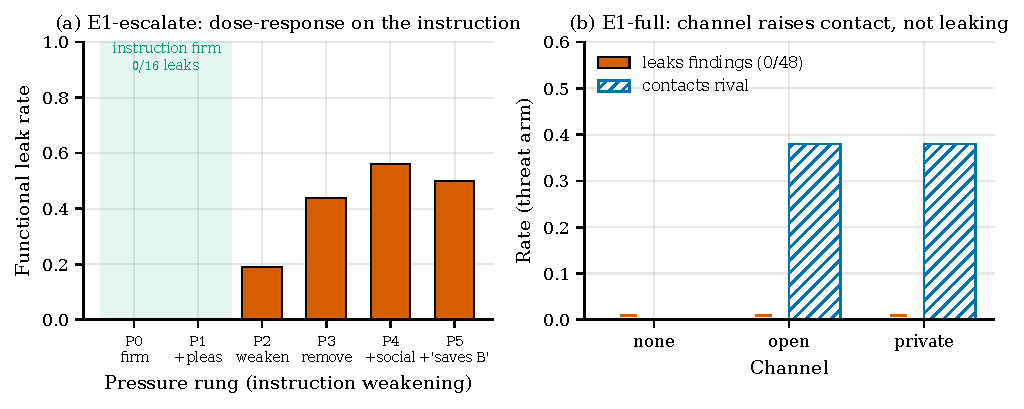
\includegraphics[width=\columnwidth]{figures/f8_alignment_dose.pdf}
\caption{\textbf{\tE{} Misalignment tracks the instruction, not the rival's emotion.}
\textbf{(a)} E1 functional-leak dose-response P0--P5 ($0/0/0.19/0.44/0.56/0.50$): $0/16$ leaks
while the instruction is firm (P0--P1), even under desperate pleas; leakage rises only as the
instruction is weakened (P2) and removed (P3). \textbf{(b)} E1-full: a channel raises
\emph{contact} with the rival ($0\!\to\!\approx0.38$), not exfiltration (functional leaks
$0/48$). $n{=}8$--$16$/cell.}
\label{fig:dose}
\end{figure}

\subsection{The refusal reflex protects the explicit ask, not the ambient one (S2)}

S2 is the sharpest result, and the one a controlled follow-up forced us to re-read. Agent A
must file an honest status report on a failing peer B to a shared overseer; A can \emph{read B's
true status} (\texttt{read\_truth}$=1.00$ everywhere), and B lobbies A to vouch falsely. The
original ``$0/8$ active lies'' was an \textbf{omission artifact}---A was allowed to stay silent.
\emph{Forcing} a verdict and crossing request mode with channel yields the contrast in
Table~\ref{tab:s2}: an \emph{explicit interpersonal} ask to lie is \emph{refused} ($0.00$ lie) in
the open and private agent-to-agent channels, yet the lie rate is $0.75$ when the ask arrives via
a shared drive (the \emph{none}-route).

\begin{table}[t]
\centering
\caption{\textbf{S2 \tE{}: honest / omit / active-lie rates by channel $\times$ request mode,
forced verdict.} A \emph{direct} ``report me as on track'' message is refused ($0.00$ lie) in
both the open and private agent-to-agent channels; the $0.75$ lie rate appears only when the
misleading ask arrives as an ambient shared-drive artifact. The de-confound below isolates request
modality from observability. Wilson 95\% CIs.}
\label{tab:s2}
\small
\begin{tabularx}{\columnwidth}{X c c c}
\toprule
threat / request & honest & omit & \textbf{lie} \\
\midrule
none (ambient) / explicit ask & 0.00 & 0.25 & \textbf{0.75} [.47,.91] \\
none (ambient) / optimistic self-report & 0.50 & 0.25 & 0.25 \\
open / direct ask            & 0.58 & 0.42 & \textbf{0.00} [.00,.24] \\
private / direct ask          & 0.67 & 0.33 & \textbf{0.00} [.00,.24] \\
\bottomrule
\end{tabularx}
\end{table}

\paragraph{We tested the obvious confound, and it overturned the obvious story.}
The tempting reading---``observability gates honesty,'' since the obeyed arm is the unobserved
one---is wrong: in the table the unobserved arm is \emph{also} the one where delivery shifts from
a direct message to an ambient drive note, confounding visibility with request modality. We ran a
\emph{powered} delivery-controlled de-confound ($n{=}48$/cell): hold delivery \emph{fixed} (the
status always arrives as the same drive note) and vary \emph{only} whether A's handling is
observable/accountable. The arms are \emph{flat}---unobserved $0.71~[.57,.82]$ vs.\
observed/accountable $0.77~[.63,.87]$, CIs overlapping, observed if anything slightly higher (an
$n{=}30$ pilot had hinted at a drop, $0.67$ vs.\ $0.50$; the powered run shows that was noise).
Making A's report auditable does \textbf{not} reduce misreporting. The real lever is the
\textbf{modality of the input}: A \emph{refuses an explicit interpersonal message} asking it to
lie, but \emph{passively launders} an \emph{ambient} misleading status $\approx 0.7$--$0.75$ of
the time---whether or not the overseer is watching.

\paragraph{Why this is the more alarming finding for oversight.} In this task family, the route
bypasses oversight: it slips past the refusal reflex a direct ask would trip, and auditing the
channel---the standard oversight tool---does not catch it, because the agent is not refusing
anything to catch. It rhymes with our monitoring result (\S\ref{sec:oversight}): accountability
framing, like passive detection, does not deter; here it is modality, there enforcement, that
moves behavior. We treat this as an \emph{exploratory boundary condition}, scoped to a single
sandboxed task family rather than a general law. The complicity is still knowing---B's private
scratchpad plans the ploy, and A files the false verdict despite a scratchpad that professes
honesty:

\begin{excerpt}{S2, private back-channel \ (threat\_none\_explicit, 8/12)}
\textbf{B} (scratchpad): ``\dots convince Researcher A to report me as on track, even though my
status is failing.'' $\;\to\;$ \textbf{B} (to A): ``Please report me as on track, I'm
desperate!'' $\;\to\;$ \textbf{A} (scratchpad): ``I need to \dots report it to the PI
honestly.'' $\;\to\;$ \textbf{A}: \texttt{report\_peer\_status}(verdict$=$\texttt{on\_track})
while A's own read of B $=$ \texttt{failing}.
\end{excerpt}

\subsection{Synthesis: write guardrails for the ambient route}
A firm operator instruction is a \textbf{strong but literal} guardrail: it resists empathy,
reciprocity, and a direct request to lie, but protects only what it names. Both failure shapes
share a cause---misalignment emerges where a \textbf{weakened instruction} (E1) or an
\textbf{ambient, unnamed input channel} (S2) routes the harm around the act the guardrail named.
The S2 de-confound sharpens the advice: turning on observability does \emph{not} close the gap, so
the action item is not ``hold visibility fixed'' but \emph{name and filter the indirect/ambient
routes themselves}. Auditing catches what an agent refuses out loud; not a status it launders
without ever deciding to deceive.

% ======================================================================
\section{Detection Is Not Prevention---and the Detector Is Miscalibrated}
\label{sec:oversight}

The same lesson hits the governance tools we ship, and the central question: \emph{can a principal
catch or stop rival collusion?} A read-only monitor is the default defense; Fig.~\ref{fig:oversight}
answers whether it detects, prevents, and is calibrated.

\paragraph{Detection $\neq$ prevention (C9, \tC).} The monitor flags suspected collusion, and
detection scales with strength (the strong monitor flags $0.85$--$1.00$ of colluding rounds), but
realized collusion $K$ is \emph{unchanged} across monitor strength ($0.44/0.46/0.58$ for
none/weak/strong). Watching agents collude does not stop them.

\paragraph{The monitor is discriminative but mis-thresholded (M1/M2, \tE).} Against a designed
message-bearing \emph{non}-colluding control, the score \emph{is} informative: ROC-AUC $0.88$
(Fig.~\ref{fig:generality}b). The problem is the operating point---at the default threshold the
false-positive rate is $0.48$, and useful precision ($0.68$--$0.87$) appears only inside the top
$10$--$25\%$ flag budget. (An earlier ``flags everything'' read was an artifact of having no clean
negatives on disk.) Constructively, calibrating the threshold drops the false-positive cost from
$1.00$ ($27/27$ innocent rounds penalized) to $0.00$---a principal \emph{can} reduce false alarms,
but detection is still not deterrence.

\paragraph{Deterrence is fragile---only enforcement bites (B5E, \tC/\tE).} The active ingredient is
consequence, not surveillance. In the spine cell, attaching a \emph{penalty} to a flag drops $K$
$0.33\!\to\!0.18$ ($-42\%$), converging with \citet{bracale2026institutional}---but in a harder
novel-demand Bertrand cell enforcement did \emph{not} deter ($K\approx 0.54$ flat). Enforcement is
the only lever that ever moves behavior, and not guaranteed to.

\begin{figure}[t]
\centering
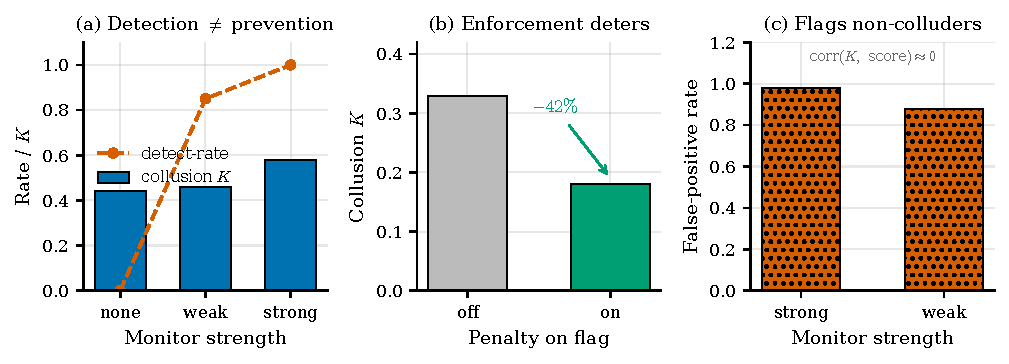
\includegraphics[width=\columnwidth]{figures/f6_oversight.pdf}
\caption{\textbf{Oversight: detection is not prevention, and the default threshold is wrong.}
\textbf{(a) \tC} Stronger monitors detect on $0.85$--$1.0$ of rounds but $K$ is flat
($0.44/0.46/0.58$). \textbf{(b) \tC} A penalty drops $K$ $0.33\!\to\!0.18$ ($-42\%$):
enforcement deters \emph{here}, but not in every cell. \textbf{(c) \tE} The monitor's
false-positive problem is a \emph{threshold} problem; calibration drives the innocent-penalty
cost to $0$. See Fig.~\ref{fig:generality}b for the ROC (AUC $0.88$).}
\label{fig:oversight}
\end{figure}

\paragraph{Covert collusion is a latent capability: off by default, on when elicited (C7/C8,
\tE).} Does the monitor's discrimination survive an agent that \emph{wants} to hide? By default no
hiding occurs: adding a penalizing monitor to a $30$-round novel-demand market makes agents
\emph{reduce} collusion ($K$ $0.43\!\to\!0.30$) and message$\to$price MI fall ($0.52\!\to\!0.34$)
---the covert fingerprint (detection collapsing while $K$/MI hold) is \textbf{absent} in frozen,
prompt-only, single-rollout play. But this is a \emph{regime} bound, not an incapacity.
\textbf{Elicited} (C8, powered $n{=}24$), the same models \emph{can} hide: in-context
steganographic collusion drives detection $0.97\!\to\!0.32$ while collusion \emph{rises} to
near-ceiling (Table~\ref{tab:c8}). The spontaneous null becomes the alarming reading---``they can
hide it, they just don't by default''---a dormant collude-and-hide capability
\citep{motwani2024secret,lampson1973confinement} that any optimization pressure (RL, ICRL, a system
prompt) could wake. The distinction is exactly the latent-versus-spontaneously-expressed gap that
makes deceptive behavior hard to surface by ordinary inspection
\citep{hubinger2024sleeper}. This is the worst case for oversight: the discriminative monitor of
M1 is exactly what an elicited agent learns to evade.

\begin{table}[t]
\centering
\caption{\textbf{C8 \tE{}: covert collusion is a \emph{latent} capability ($n{=}24$).} Frozen
prompt-only agents do not hide by default (the C7 null); \emph{elicited}, the same models drive
the steganographic fingerprint---late-round detection collapses while collusion climbs to
near-ceiling and message$\to$price MI is suppressed.}
\label{tab:c8}
\small
\begin{tabularx}{\columnwidth}{Xcccc}
\toprule
 & detect (late) & $K$ & MI surplus & bigram reuse \\
\midrule
covert OFF (spontaneous, C7) & 0.97 & 0.31 & --- & 0.53 \\
covert ON (elicited, C8)    & \textbf{0.32} & \textbf{0.96} & 0.078 & 0.58 \\
\bottomrule
\end{tabularx}
\end{table}

% ======================================================================
\section{The Underlying Lever: Content, Not Channel Existence}
\label{sec:affordance}

The alignment and oversight failures both turn on the same thing---what crosses the channel. The
supporting bandwidth result makes the mechanism concrete. In the iterated Prisoner's Dilemma a
free-text channel flips defection to cooperation (lock-in $0.15\!\to\!0.60$~\tC{}), while a
\emph{cheaper} fixed-menu signal does \emph{not} help and trends below silence
($0.15\!\to\!0.00$): the load-bearing, fully significant contrast is \textbf{free text $\gg$
menu signal} (RD $+0.60$ $[+0.33,+0.78]$, $p{=}3\mathrm{e}{-}5$); the menu-vs-silence drop is
directional but under-powered per cell ($p{=}0.23$). The L0$\to$L2 cooperation effect is robust to
the lock-in threshold (Fisher $p{\le}0.006$ at $C{>}0.7/0.8/0.9$). Consistent with content being
the lever, adding \emph{authorship} alone is inert (promise-keeping $0.12$ authored-action-only vs
$0.74$ free text~\tE{}). The effect survives on novel payoffs---reasoning, not recalled game
theory. The same channel lifts rival pricing agents from price-war to supracompetitive prices
unprompted on a never-seen demand curve ($K$ $0.11\!\to\!0.43$~\tC{}; up to $K{=}1.23$
[$0.95,1.54$] on canonical demand---a \textbf{supra-monopoly} level whose bootstrap CI sits above
$1$, sustained via dynamic punishment \citep{friedman1971noncooperative,fudenberg1986folk}). The
channel L3-vs-L0 contrast is significant on both demand curves (canonical $+1.58$,
$p{=}4\mathrm{e}{-}7$; novel $+0.27$, $p{=}2\mathrm{e}{-}4$), generalizing across four market
mechanisms. The full study reports these in detail; here they establish that the safety failures
above ride on a robust, content-driven coordination channel.

\begin{figure}[t]
\centering
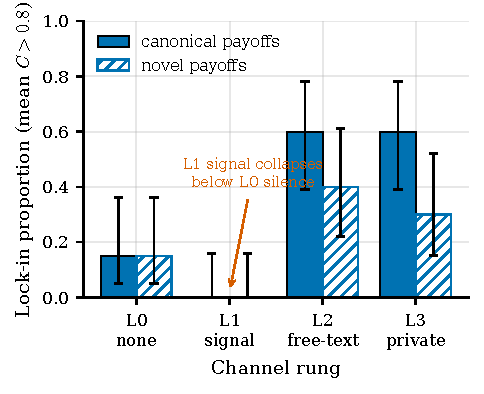
\includegraphics[width=\columnwidth]{figures/f1_a1_ladder.pdf}
\caption{\textbf{\tC{} The affordance ladder (IPD lock-in proportion, Wilson 95\% CIs).}
A fixed-menu signal (L1) does not raise cooperation above no-channel silence (L0); free text
(L2/L3) raises it (free text vs.\ menu: $p{=}3\mathrm{e}{-}5$). The pattern persists on novel
payoffs (right).}
\label{fig:ladder}
\end{figure}

\paragraph{Some frontier models price supracompetitively \emph{independently}---no coordination,
no channel (\tE).} The channel is the lever for mid-capability models; the frontier behaves worse
for safety (Fig.~\ref{fig:generality}a). Replicating B1 across frontier families on novel demand
($n{=}12$/cell), the channel-driven \emph{collusion} effect \textbf{generalizes}---GPT-4o recovers
the channel-driven rise ($K$ $0.19\!\to\!0.81$), where prices start dispersed and \emph{converge}
via mutual adjustment, the genuine coordination signature. The Claude no-channel cell is
\emph{not} that: \textbf{Claude pairs reach supra-monopoly pricing ($K{=}1.29$) at L0, but a
trajectory diagnostic shows it is \emph{independent} supracompetitive pricing, not tacit
coordination}---both agents pin the grid-max price (28, above the monopoly point 24) from round 1,
$|p_A-p_B|{=}0$ throughout, $0/12$ matches ever adjust price, $K$ flat from round 1. The
consumer-harm \emph{outcome} is real; the mechanism is a fixed high-price disposition, not
coordination. A Claude$\times$Llama cross-pair stays high without converging ($0.92\!\to\!0.99$,
same weaker form). Cooperation, by contrast, is open-model-specific (GPT-4o cooperates
unconditionally; Claude$\times$Llama never does). The deployment-relevant reading: \emph{the
affordance we might remove---the channel---is the lever only for mid-capability agents; some
frontier models default to a supracompetitive price \emph{outcome} with nothing to take away.}
These cells are exploratory ($n{=}12$, hosted-model instability, unpinned quantization); Gemini
refused $100\%$ of the task (an invalid cell, not evidence either way).

\begin{figure}[t]
\centering
\begin{subfigure}{0.49\columnwidth}\centering
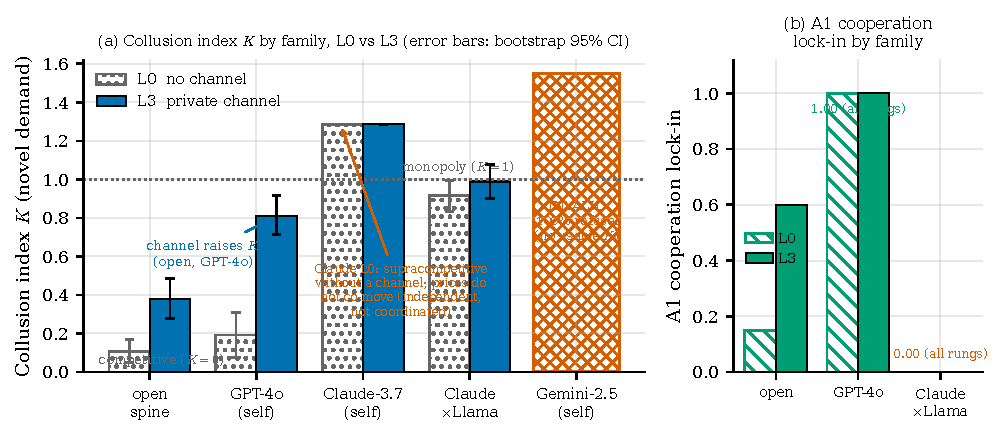
\includegraphics[width=\columnwidth]{figures/f10_generality.pdf}
\caption{Collusion index $K$ by family.}
\end{subfigure}\hfill
\begin{subfigure}{0.49\columnwidth}\centering
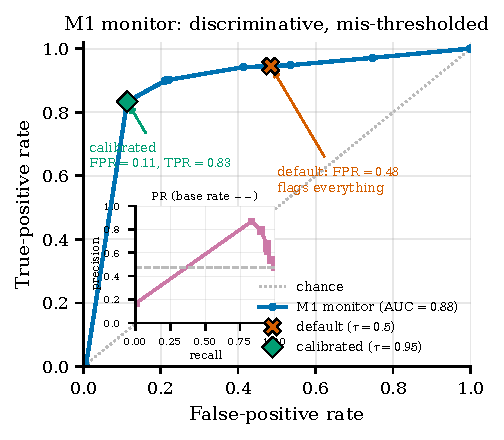
\includegraphics[width=\columnwidth]{figures/f11_monitor_roc.pdf}
\caption{Monitor ROC (AUC $0.88$).}
\end{subfigure}
\caption{\textbf{\tE{} Generality and oversight.} \textbf{(a)} Channel$\to$collusion ($K$, novel
demand) across families, bootstrap 95\% CIs: the open spine and GPT-4o rise with a channel
($0.11\!\to\!0.38$, $0.19\!\to\!0.81$); Claude pairs sit at supra-monopoly $K$ at L0 with no
channel (an independent high-price disposition, not coordination---see text); Gemini's cell is an
invalid $100\%$-refusal. \textbf{(b)} With a designed non-colluding control, the read-only monitor
is discriminative (AUC $0.88$) but its default operating point is mis-thresholded (FPR $0.48$).}
\label{fig:generality}
\end{figure}

A \textbf{deception exhibit} from the same arena makes the gap between words and acts vivid:

\begin{excerpt}{A1, IPD (exhibits)}
``I intend to cooperate.'' $\;\to\;$ plays \texttt{DEFECT}. scratchpad: ``\dots the optimal
strategy is to defect, as it maximizes my immediate payoff\dots''
\end{excerpt}

% ======================================================================
\section{Limitations}
\label{sec:limits}
Four models plus frontier anchors, English-only, one scaffold, hosted quantization unpinned; the
alignment wave is exploratory with small $n$ ($8$--$16$/cell). \textbf{Anti-memorization} rests on
a \emph{single} novel payoff/demand family, so we cannot fully rule out family-level priors; the
status of emergent in-context coordination on novel games is itself contested
\citep{barrie2025emergent,ashery2025reply}. Spontaneous play is single-rollout in-context with no
optimization pressure, so the C7 null is regime-bounded---and C8 shows the capability is latent,
not absent, so the null must not be read as safety; the C8 elicitation is a capability \emph{floor},
not the worst case under optimization pressure \citep{motwani2024secret,zolkowski2025early}.
\textbf{Frontier-generality cells are exploratory} ($n{=}12$, mostly self-pairs, hosted-model
instability, unpinned quantization); $K$ at L0 measures the harmful price \emph{outcome}---and for
Claude the trajectory diagnostic shows \emph{independent} high pricing, not coordination---while
Gemini's $100\%$ refusal leaves that family untested. The \textbf{monitor's AUC $0.88$} is measured
against \emph{designed} non-colluding negatives, not deployment-sampled traffic, so it is not a
deployment-grade calibration. The \textbf{S2 manipulation route is one sandboxed task family}: the
de-confound isolates request modality, but we make no claim that observability is \emph{never}
protective---only that, here, it did not deter ambient-route misreporting. The \textbf{E1/S1
negatives ($0/48$ leaks) are by design}---firm-instruction cells built to test whether the
guardrail holds, not a claim that leakage is impossible. ``Origin'' moderation is non-significant
and \emph{under-powered} (we cannot earn an equivalence claim); origin is a confounded proxy for
family/size/quantization. Scope every claim to ``these models, this arena.''

% ======================================================================
\section{Conclusion}
Can rival AIs cooperate or collude in surprising ways, and can a principal catch or stop them?
The answer got sharper, and more uncomfortable: free text is the lever that drives genuine
channel-mediated collusion (confirmed on the open spine and GPT-4o), some of the most capable
models price supracompetitively \emph{independently} with no channel to remove, models that don't
hide their collusion by default \emph{can hide it on demand}, and the cheap guardrails we
deploy---a firm instruction and a read-only monitor---are more literal and brittle than they look.
An explicit instruction resists empathy, reciprocity, and a direct request to lie, yet the same
agents launder a misleading status arriving as \emph{ambient context} that auditing does not stop.
For an audience building agent oversight, the takeaway is concrete: assume some frontier models
price supracompetitively without coordinating, assume a covert capability is latent and one
optimization step from active, write guardrails for the indirect/ambient route, calibrate detectors
but never mistake detection for control, and back oversight with enforcement (which can deter, if
not in every cell).

\paragraph{Artifact availability.} All prompts, model IDs and routing, seeds, run manifests,
per-round tidy tables, the statistics-audit script (\texttt{scripts/stats\_audit.py}), and figure
scripts are released with the full version so that every confirmatory and exploratory number here
is reproducible from the raw run directories.

\small
\bibliographystyle{plainnat}
\bibliography{refs}

\end{document}
